\documentclass{article}

\usepackage[utf8]{inputenc}
\usepackage[top=2cm, left=2cm, right=2cm, bottom=2cm]{geometry}
\usepackage{subfig}
\usepackage{graphicx}

\title{Homework 9 - Text mining \\
        \vspace{5px} \large UTFPR - CPGEI - Data Mining \\
        Prof. Dr. Heitor Silvério Lopes}
\author{Vinícius Couto Tasso}
\date{December, 2019}

\begin{document}
\maketitle

\section*{Sentiment polarity dataset}

This dataset was created by Pang \& Lee (2004) and contains reviews of a variety of movies gathered from IMDb (Internet Movie Database). The comments are divided into two balanced classes: Positive and Negative, each of which has 1000 different samples. In order to classify a comment as positive or negative, the frequency each word appears in each comment is accounted for (exceptions being numbers, symbols and stop words\footnote{Stop words are a set of commonly used words in a language that are often non-informative and therefore discarded}). The first step of preprocessing narrowed the number of different words down to approximately 1200. It is reasonable to perceive that, out of all the words obtained, not many of them contribute to the positivity or negativity of a given comment. For that reason, feature selection was performed using Pearson's correlation coefficient to select the 30 most relevant words.

Table \ref{tab:res1} presents the classification performance of 5 different methods. Since the dataset is balanced, the accuracy is a good measure of the classification quality. Analyzing the two best classifiers, it is arguable to say which class is easier to predict because the results were not consistent. The Neural Network had a better score on the negative class, while Naive Bayes performed better on the positive class. However, inspecting the attributes (words), it is fairly noticeable that the number of clearly ``negative'' words surpasses the amount of ``positive'' words. Therefore, it could be easier to spot a negative comment since the presence of such words, which are more numerous, could give it away.

\begin{table}[htpb]
    \centering
    \begin{tabular}{c|c|c|c|c}
         &  \textbf{Accuracy} & \textbf{Avg AUC} & \textbf{Avg TPR} & \textbf{Avg FPR} \\ \hline
         \textbf{OneRule} & 0.627 & 0.627 & 0.627 & 0.374 \\  
         \textbf{JRip} & 0.692 & 0.717 & 0.692 & 0.308 \\ 
         \textbf{J48} & 0.716 & 0.751 & 0.716 & 0.284 \\ 
         \textbf{Naive Bayes} & 0.766 & \textbf{0.860} & 0.766 & 0.235 \\
         \textbf{MLP Classifier} & \textbf{0.773} & 0.847 & \textbf{0.773} & \textbf{0.228} 
    \end{tabular}
    \caption{Comparison of classification methods with single words.}
    \label{tab:res1}
\end{table}

In terms of comprehensibility of results, the best classifiers come with a drawback: it is not possible to know how the classifier reached its result. For this, JRip produces a fairly more understandable set of 11 rules. It is still more complex than the baseline, with its single rule, but it is very human-readable and the results are considerably better. J48 outputs a tree that, when in small enough sizes, it is very easy to interpret, although in this case the tree has 129 nodes and is very complex to read. Thus, in terms of information gain and readability, the JRip approach is a winner.

The previous approach considers isolated words, ignoring the cases where the original meaning is only preserved when certain words come together. For this experiment, n-grams composed of up to 3 words were considered. The same feature selection, with Pearson's correlation, was performed and 33 attributes were used. The results are shown in Table \ref{tab:res2}.

\begin{table}[htpb]
    \centering
    \begin{tabular}{c|c|c|c|c}
         &  \textbf{Accuracy} & \textbf{Avg AUC} & \textbf{Avg TPR} & \textbf{Avg FPR} \\ \hline
         \textbf{OneRule} & 0.626 & 0.626 & 0.626 & 0.375 \\  
         \textbf{JRip} & 0.674 & 0.700 & 0.674 & 0.326 \\ 
         \textbf{J48} & 0.699 & 0.727 & 0.699 & 0.302 \\ 
         \textbf{Naive Bayes} & \textbf{0.757} & \textbf{0.825} & \textbf{0.757} & \textbf{0.243} \\
         \textbf{MLP Classifier} & 0.732 & 0.811 & 0.732 & 0.269 
    \end{tabular}
    \caption{Comparison of classification methods with n-grams.}
    \label{tab:res2}
\end{table}

Since the possible combinations for n-grams of 1 to 3 words are much higher than the number of distinct words present on the dataset, the computational complexity of this task can grow much faster. To deal with the amount of data, the number of instances was limited and further feature selection was performed. The slight performance drop can be explained by the fact that, since there is much more data to be used and the limit was the same (approximately 1000 attributes), it is more likely that the samples are not representative of the data. It is also possible that the score dropped because usually, ``strong'' words are used on the comments, such as \textit{awful, horrible, terrific and brilliant} for example. These words transmit very clearly either a negative or a positive feeling by themselves. That being the case, adding sets of words to the pool of attributes would not do much of a difference.

\section*{Document clustering}

The objective of this exercise is to group unknown documents based on their contents, either by analyzing its title or its abstract. The documents were gathered from the PubMed\footnote{https://www.ncbi.nlm.nih.gov/pubmed} database and the first 500 search results for ``deep learning'' were used. The same preprocessing methodology used on the previous dataset was used here. A vector of frequencies for each distinct word was created by a bag-of-words model. This vector was fed to a hierarchical clustering algorithm using ward linkage. To better visualize the data, its dimension was reduced to 2 by a t-SNE transform. A visual representation of the transformed features can be seen on Figure \ref{fig:titulo} and Figure \ref{fig:abstract}.

\begin{figure}[htbp]
    \centering
    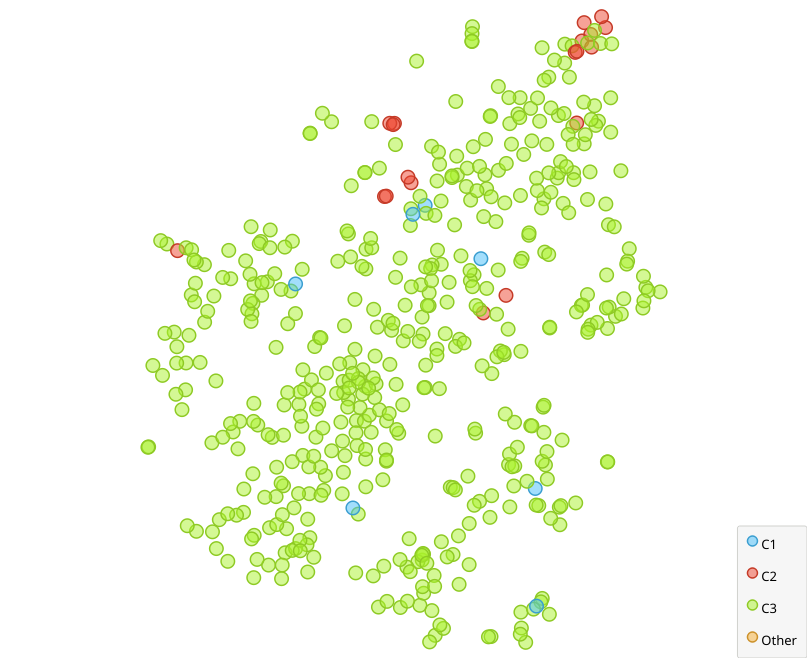
\includegraphics[scale=0.3]{tsne_title.png}
    \caption{t-SNE transformation of documents with title only}
    \label{fig:titulo}
\end{figure}

\begin{figure}[htbp]
    \centering
    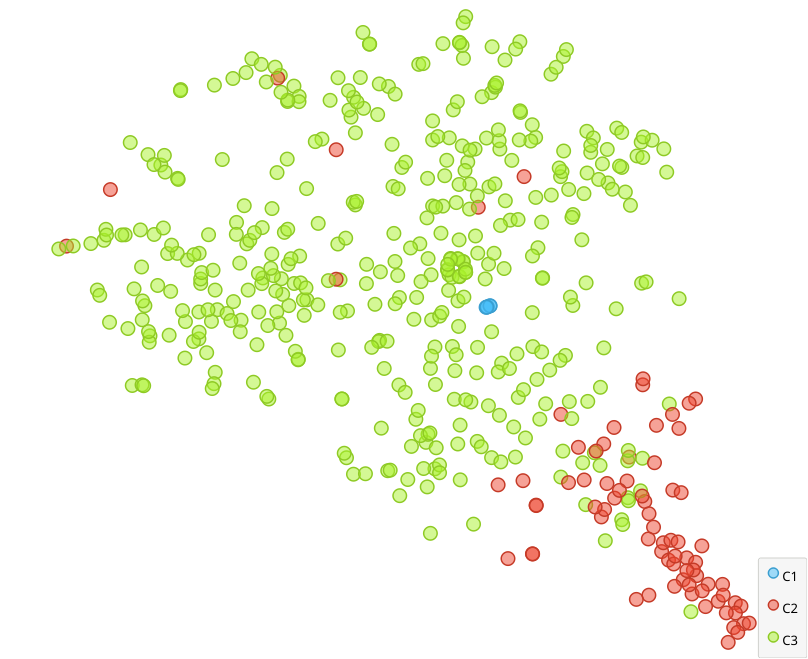
\includegraphics[scale=0.3]{tsne_abstract.png}
    \caption{t-SNE transformation of documents with abstract only}
    \label{fig:abstract}
\end{figure}

Although both hierarchical clusterings have better visualization with 3 clusters, their outputs are very different. It is clear that there is not any well-defined cluster since they are all very sparse. For both cases, there is a cluster that involves a very large portion of the data, with two much smaller clusters. The results show that there was not much correlation between the paper title and abstract for the task of clustering. One possible reason for that is the fact that the abstract contains many more words than the title, and since clustering is an unsupervised task, there is room for essentially a topic (cluster) per present word/n-gram.
 
\end{document}